\documentclass[]{article}

\usepackage[utf8]{inputenc}

\usepackage{fullpage}
\usepackage{graphicx}

\usepackage[french]{babel}

\usepackage{times}
\usepackage[colorlinks=true]{hyperref}
\usepackage{color}
\usepackage{titling}
\usepackage{subfig}
\usepackage{chngpage}
\usepackage{calc}

%-- Logos PDG --
\pretitle{
\begin{center}

\begin{figure}[!tbp]
  \centering
  \subfloat{
\includegraphics[width=0.25\textwidth]{UMons_logo.png}}
  \hfill
  \subfloat{
\includegraphics[width=0.25\textwidth]{sciences_logo.png}}\\
\end{figure}
~\newline

}

\posttitle{\end{center}}

\begin{document}

\title{
\vspace{1.6cm}
{\Huge Big Data Analytics I}\\
\vspace{0.5cm}
{\Huge Rapport de projet}\\
}
\bigskip


\author{
\Large{Sam Boosko}\\
\Large{Rémy Decocq}\\
\Large{Dimitri Waelkens}
}

\date{
\vspace{9.5cm}
Année Académique 2018-2019\\
Master en Sciences Informatiques\\
Faculté des Sciences, Université de Mons}

\maketitle          

\thispagestyle{empty}   

\newpage

\section{Introduction}

La jeu de données fourni a été construit lors de campagnes marketing menées par un organisme bancaire, sous la forme d'appels téléphoniques vers de potentiels clients. Pour chaque personne sondée, il est renseigné si oui ou non, à la suite de cet appel, elle a souscrit à un dépôt bancaire à long terme dans ladite banque. Le but de la compétition est de prédire si ce sera le cas pour de nouveau client en se basant sur des variables mesurées identiques. Le jeu d'entrainement contient 30436 observations (dont le résultat "a souscrit" est connu et est repris par la variable $y$), tandis ce que le jeu de test (dont le $y$ nous est sciemment pas communiqué) est séparé en deux et contient au total $10182 \times 2 = 20364$ mesures.

\par Les données sont des mesures de variables de deux types : celles relatives au client lui-même (données personnelles) et celles relatives aux potentiels sondages sur le client durant les campagnes. On a donc :\newline
~\\
\vspace{0.2cm}
\textbf{Variables explicatives}\\
\vspace{0.1cm}
\indent \texttt{Persos} :
\begin{itemize}
\item[$\bullet$] \textit{age}, (type de) \textit{job}, statut civil \textit{marital}, niveau du milieu d'éducation \textit{edu}
\item[$\bullet$] \textit{default} a une défaillance de crédit, \textit{housing} sous prêt immobilier, \textit{loan} a un prêt personnel
\end{itemize}
~\\
\indent \texttt{Campagnes} :
\begin{itemize}
\item[$\bullet$] \textit{contact}, \textit{month}, \textit{day\_of\_week} : type de communication, mois et jour de la semaine du dernier contact
\item[$\bullet$] \textit{campaign} : nombre de contacts établis durant la campagne correspondant au jeu de données
\item[$\bullet$] \textit{pdays} : nombre de jours passés depuis le dernier contact d'une campagne précédente
\item[$\bullet$] \textit{previous} : nombre de contacts déjà établis avant cette campagne
\item[$\bullet$] \textit{poutcome} : résultat pour ce client suite à la campagne précédente
\end{itemize}


~\\
\textbf{Variable expliquée}\\
\indent $\; \bullet$ \textit{y} : le client a ouvert un dépôt à long terme dans l'organisme bancaire

\section{Méthodologie}

\subsection{Analyse des variables et observations}

Une variable que l'on peut remettre en question serait \textit{default}. Effectivement, si on regarde la proportion des valeurs pour cette variable catégorique, on a 75.24\% de 'no', 24.74\% de 'unknown' et moins de 0.01\% de 'yes' (3 observations). Une variable qui est presque binaire de la sorte avec une valeur à la sémantique inconnue apporte de la confusion et ne permet pas d'expliciter rationnellement une information. Elle sera donc omise.\\

\par Un autre problème peut être mis en avant pour la variable \textit{pdays}. Bien qu'elle soit numérique, une valeur de 999 renseigne 'le client n'a jamais été contacté dans une campagne précédente' (et donc le nombre de jours passés depuis le contact lors de la dernière campagne est indéterminé). On utilise donc une valeur numérique pour signifier quelque chose qui n'est pas quantifiable (au contraire des valeurs pour les clients déjà contactés qui s'étendent de 0 à 11 jours). Un compromis pour avoir une meilleure sémantique serait une variable catégorique, considérant 'recent' si le nombre de jours est $<6$, 'late' s'il est $\geq 6$ et 'never' pour les valeurs 999. Notons que cela se fait au prix d'une perte d'information, mais le nombre conséquent d'observations pour lesquelles \textit{pdays} vaut 999 (30329) nous y motive.\\

\par On constate également des incohérences en considérant la variable $previous$ avec $pdays$. Théoriquement, si $pdays=999$, alors le client n'a jamais été contacté donc $previous$ (indiquant le nombre de contacts ultérieurs toutes campagnes confondues) doit valoir 0. Or, 1316 observations ne satisfont pas ce prédicat (soit 4\% du jeu de données) parmi lesquelles 108 ont un réponse positive pour la variable expliquée \textit{y}. Ces observations sont importantes, effectivement seulement 2342 parmi les 28094 observations affichent une réponse positive pour \textit{y}. Pour que notre modèle soit efficace, il faut pouvoir tenir compte de toutes ces précieuses observations.


\subsection{Sélection du type de modèle}

Comme les prédictions à faire sont sur la variable \textit{y} qui est binaire, on s'intéresse aux méthodes de classification. Trois approches ont été considérées : LDA, la Régression Logistique et les Arbres de décision. La première semble assez peu adaptée : nous ne pouvons pas affirmer rentrer dans ses hypothèses de distribution gaussienne sur les prédicteurs et de séparation claire des classes, qui ne seraient qu'au nombre de 2 (ce qui n'exploite pas la force de LDA). La seconde a été sélectionnée dans un premier temps, dans l'optique d'en améliorer les résultats avec les méthodes de Bagging en implémentant les arbres par la suite si le temps le permettais. Effectivement, la \textbf{Régression Logistique} semble toute indiquée pour notre problème : variable expliquée binaire, correspondance avec la fonction d'erreur \textit{LogLoss} utilisée pour évaluer nos résultats, dummification des variables catégoriques aisée.

\subsection{Sélection des prédicteurs pertinents}

Une fois les premiers modèles construits, il est apparu évident que certaines variables n'y étaient vraiment pas significatives. Afin de sélectionner un ensemble optimal de variables apportant de l'information au modèle parmi les 14 disponibles, les technique de \textbf{Stepwise Selection} est employée. En l'opérant dans les deux sens, cela permet de déduire un ensemble fort de variables importantes sur lesquelles reconstruire le modèle de régression logistique.

\subsection{Séparation du jeu de données}

Comme énoncé à la section 2.1, seulement 2342 observations présentent une réponse positive, ce qui ne constitue que 7\% du jeu total. Notre modèle risque de ne pas les prendre suffisamment en compte car noyés dans la masse (ie. le modèle overfit sur des observations majoritairement telles que $y=0$). Construire le modèle sur un jeu plus balancé pourrait offrir de meilleurs résultats. Une méthode est donc mise en œuvre pour séparer le jeu de données en \textit{training}/\textit{validation} \textit{sets }tout en tenant compte de cela, dont la procédure est :\\
~\\
\indent \texttt{SepDataset}, paramètres numériques \textit{prop\_ok} et \textit{balance}  
\begin{enumerate}
\item Diviser le set en \textit{obs\_no} et \textit{obs\_ok} respectivement les observations telles que y=0 et y=1 
\item Constituer le \textbf{validation set}: prendre $\frac{size(obsok)}{prop}$ observations de \textit{obs\_ok} et un même nombre dans \textit{obs\_no}
\item Considérer \textit{obs\_remaining} l'ensemble des observations n'étant pas dans le \textbf{validation set}, prendre parmi elles toutes les observations y=1 qu'on désigne par \textit{obs\_remaining\_ok} 
\item Constituer le \textbf{training set}: l'union de \textit{obs\_remaining\_ok} et \textit{size(\textit{obs\_remaining\_ok})} $\times$ \textit{balance} observations de l'ensemble \textit{obs\_remaining} telles que y=0
\end{enumerate}
~\\
On obtient alors un validation set de taille limitée contenant $\frac{size(obsok)}{prop} \times 2$ observations, dont la moitié sont telles que y=1 et l'autre y=0. Le training set contient d'une part toutes les observations restantes du set telles que y=1, et d'autre part un nombre d'observations telles que y=0 égal à \textit{balance} $\times$ la taille de cet ensemble. Donc plus \textit{balance} est faible, plus il y aura un nombre équivalent de y=0 et y=1 dans le training set. Le training et validation set sont bien distincts.

\subsection{Validation du modèle}

Afin de vérifier la cohérence de notre modèle et estimer l'erreur de test, ainsi que d'autres statistiques en découlant, la \textbf{Cross-Validation} est la méthode qui est employée. La procédure se présente de cette façon :
~\\
\indent \texttt{CrossValidate}, paramètres entiers \textit{nbrCV} et \textit{nbrFolds}
\begin{enumerate}
\item itérer de 1 à \textit{nbrCV} en générant \textit{nbrFolds} partitions du dataset aléatoirement à chaque fois
\item Dans chaque itération, itérer sur chacun des \textit{nbrFolds} en le considérant comme l'ensemble de test, et appliquant \texttt{SepDataSet} sur l'ensemble formé par les \textit{nbrFolds-1} autres
\item Lancer le modèle avec les prédicteurs fixés sur l'ensemble de training retourné par \texttt{sepDataSet}, évaluer l'erreur sur l'ensemble de test (le fold courant)
\item Calculer une moyenne des erreurs sur les \textit{nbrFolds} itérations, à partir des \textit{nbrCV} moyennes ainsi calculées, afficher leur distribution et en calculer les moments
\end{enumerate}

\newpage

\section{Résultats et discussion}

Ci-dessous le résultat du fitting du modèle de régression logistique en utilisant la combinaison de variables déduites comme les plus explicatives par les procédures de sélection stepwise :

\begin{figure}[!ht]
   \begin{adjustwidth}{-\oddsidemargin-1in}{-\rightmargin}
     \centering
     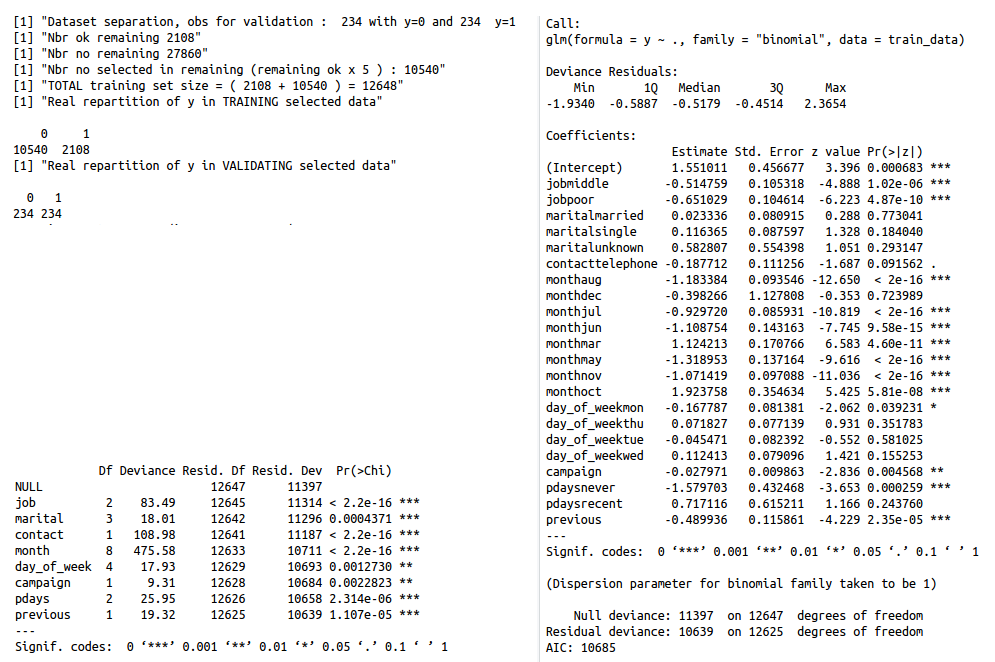
\includegraphics[width=\paperwidth - 1cm]{callglm}
   \end{adjustwidth}
\end{figure}
\vspace{0.3cm}
Ce modèle fait l'hypothèse que la relation avec la variable expliquée est linéaire. Pour se faire une idée de ses performances, on peut calculer les prédictions qu'il fournit sur d'une part les données du training set (dont le résultat sera donc sujet à de l'overfitting) et d'autre part sur le validation set (qui contient donc un nombre équivalent d'observations telles que y=0 et y=1). On en sort les mesures suivantes, avec matrices de confusion (les colonnes étant les vraies valeurs et les lignes les valeurs prédites) :

\begin{figure}[!ht]
   \begin{adjustwidth}{-\oddsidemargin-1in}{-\rightmargin}
     \centering
     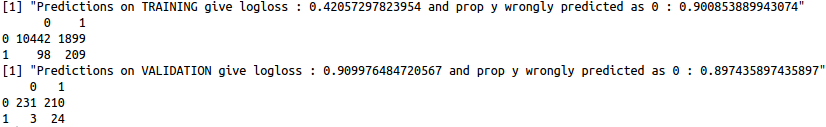
\includegraphics[width=\textwidth]{confmat}
   \end{adjustwidth}
\end{figure}

\newpage

Cette classification a été effectuée considérant un seuil de 0.5 (au dessus de cette probabilité prédite, y=1). Afin d'expliciter les distributions des probabilités qui sont les prédictions sur différents sets (y compris l'ensemble réel de test hors validation), des boxplots sont utilisés. Comme les faux négatifs semblent visiblement être le point faible du modèle, on en renseigne également la proportion pour chaque set dont on connaît les vraies valeurs de y. Pour le test set, on se contente d'afficher la proportion des prédictions qui mènent à considérer une réponse positive y=1.
\begin{center}
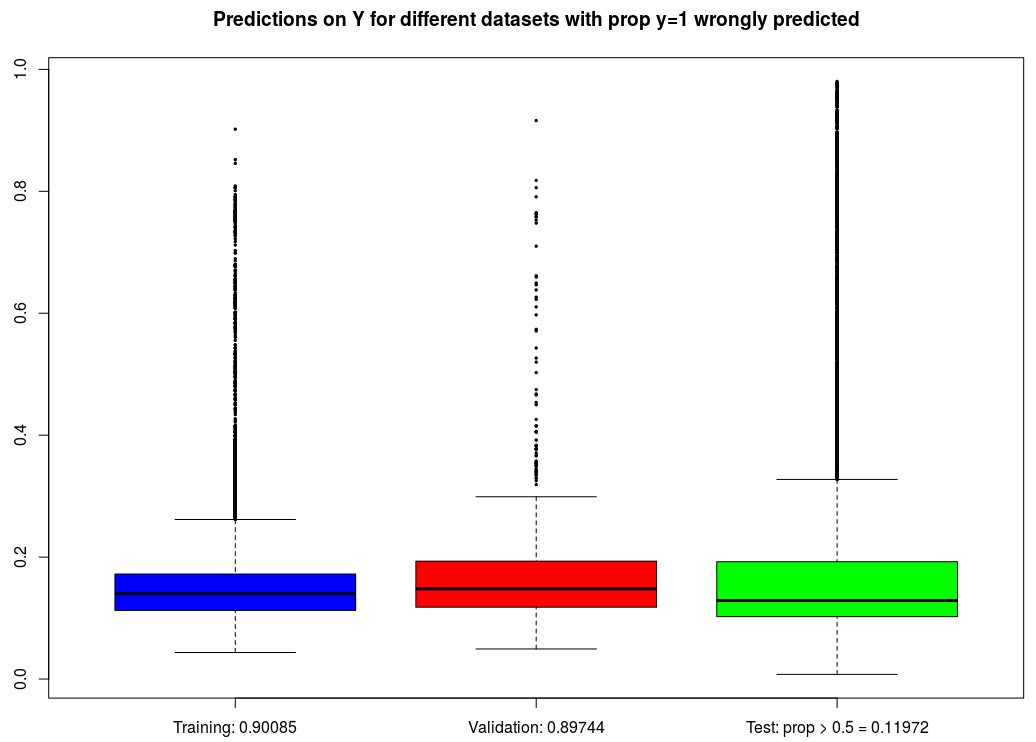
\includegraphics[scale=0.35]{pred_distrib}
\end{center}

À noter que ce modèle a été fit et validé sur des ensembles tels que obtenus par un appel à la procédure \texttt{SepDataSet} avec les paramètres \textit{prop=10} et \textit{balance=5}. Il y a donc dans le training set toutes les observations telles que y=1 n'étant pas dans le validation set et une proportion de $5 \times$ d'observations y=0. Afin de mieux visualiser le lien entre le paramètre \textit{balance} et l'efficacité du modèle entrainé vis-à-vis de la LogLoss, des moyennes sont calculées sur plusieurs utilisations de \texttt{SepDataSet} par valeur de balance (avec un nombre d'observations du validation set fixé par le paramètre \textit{prop} à 10). On visualise également les distributions des prédictions sur le test set par de tels modèles :

\begin{figure}[!ht]
   \begin{adjustwidth}{-\oddsidemargin-1in}{-\rightmargin}
     \centering
     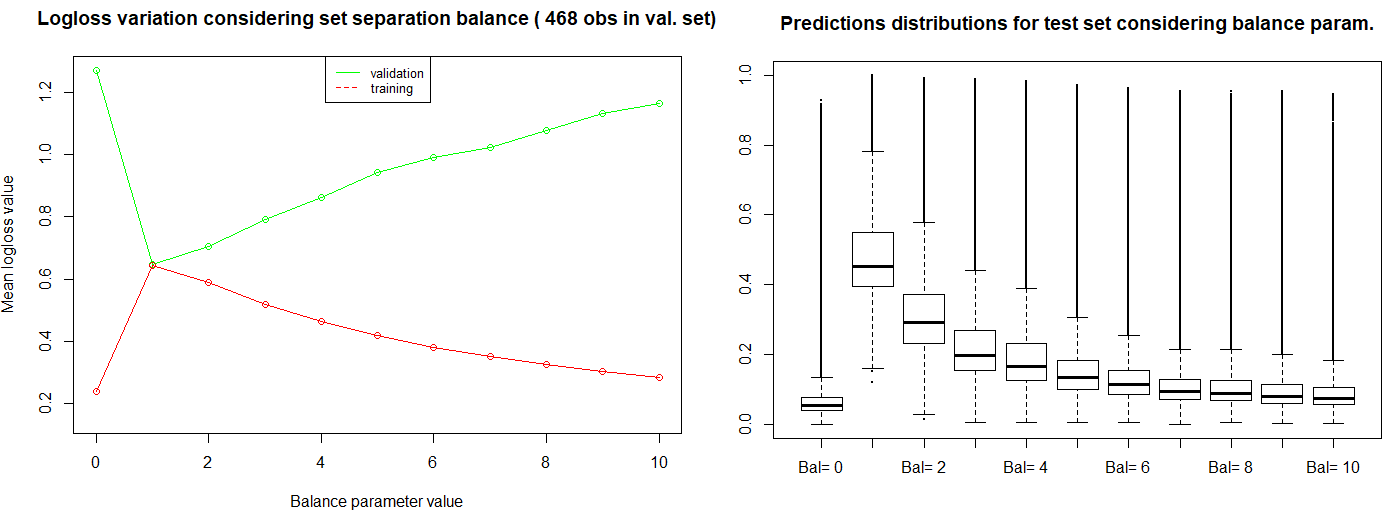
\includegraphics[width=\textwidth]{balance_both}
   \end{adjustwidth}
\end{figure}

\newpage

La procédure de cross-validation va permettre d'estimer l'erreur de test et de mettre en évidence la stabilité du modèle. À chaque fold, on retient 3 mesures : l'indicateur AIC du modèle construit, la valeur de la fonction d'erreur LogLoss par rapport à son application sur le test set du fold et la proportion de faux négatifs sur les réponses qui en sortent. Il s'agit de moyenne sur 10 runs où le jeu de données était partitionné en 10 folds (appel à \texttt{CrossValidate} avec \textit{nbrCV}=10 et \textit{nbrFolds}=10, donc \textit{size(trainingset)} $\approx$ 11300 et \textit{size(testset)} $\approx$ 3040), l'aspect aléatoire résidant dans la sélection des observations de \texttt{SepDataSet}.


\begin{figure}[!ht]
   \begin{adjustwidth}{-\oddsidemargin-1in}{-\rightmargin}
     \centering
     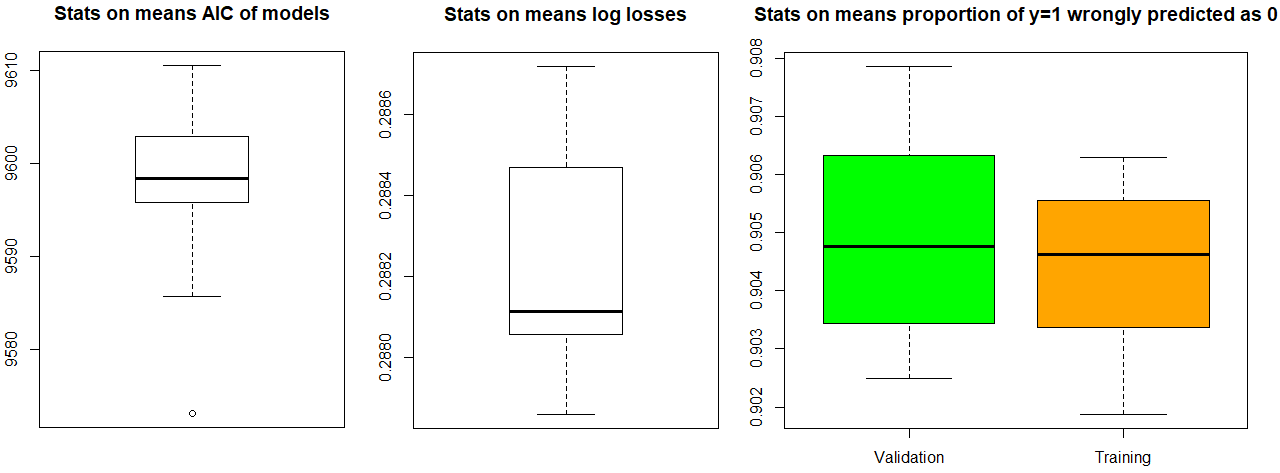
\includegraphics[width=\textwidth]{cv2}
   \end{adjustwidth}
\end{figure}

\vspace{-1cm}
\section{Conclusion}

Après avoir appliqué la \textit{stepwise selection} et déterminé quelles variables semblaient significative sous une hypothèse linéaire, nous avons évalué le modèle sur le training et validation set, et prédit les probabilités sur l'ensemble de test. Le fait que la logloss obtenue sur le validation set soit si élevée est dû à la proportion équivalente d'observations telles que y vaut 1 et 0, et la faible taille de cet ensemble (on se met donc en quelque sorte "dans le pire cas"). On a illustré le fait qu'en augmentant la taille du training set avec des observations telles que y=0, la logloss augmente mais la variance de la sortie \textit{y} diminue, un bon compromis étant la valeur 5 pour \textit{balance} (si \textit{prop} est fixé à 10). Selon les résultats des prédictions mises en ligne, procéder de la sorte à une séparation balancée du dataset nous a permis de faire descendre la logloss de 0.55 à 0.52.\\

\par La validation croisée apporte des informations sur la façon dont le modèle se comporte quand il est construit et testé sur différentes parties du jeu de données dont on dispose. Globalement, les résultats sont assez constants et la proportion de faux négatifs reste importante, de l'ordre de 90\%. Finalement, en réappliquant le modèle de régression logistique avec les variables sélectionnées sur un ensemble de training tel que retourné par \texttt{SepDataSet} avec \textit{balance}=5 et \textit{prop}=10, les prédictions ont la distribution suivante :

\begin{center}
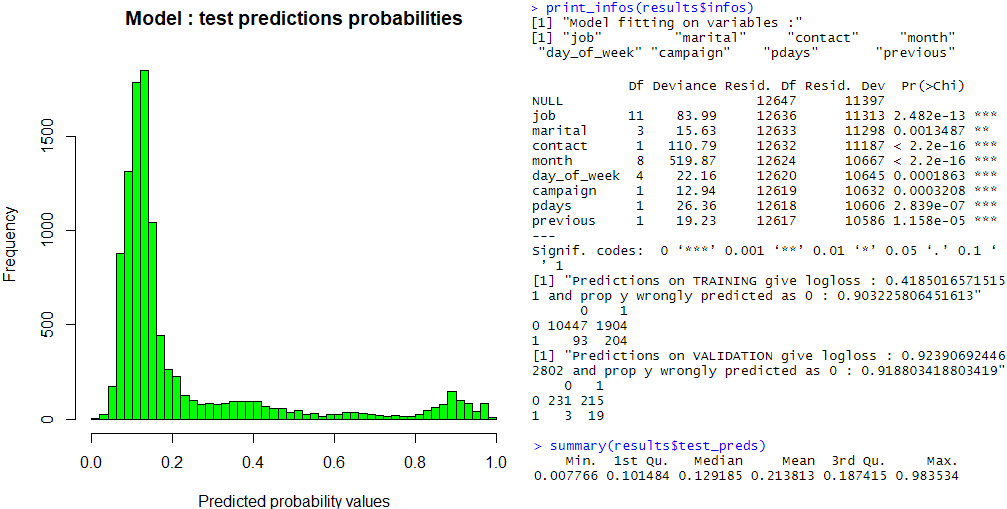
\includegraphics[height=5.75cm]{preds_test}
\end{center}

\end{document}